\documentclass[10pt,conference]{IEEEtran}
\IEEEoverridecommandlockouts
% The preceding line is only needed to identify funding in the first footnote. If that is unneeded, please comment it out.
\usepackage{cite}
\usepackage{amsmath,amssymb,amsfonts}
\usepackage{algorithmic}
\usepackage{graphicx}
\usepackage{textcomp}
\usepackage{xcolor}
\def\BibTeX{{\rm B\kern-.05em{\sc i\kern-.025em b}\kern-.08em
    T\kern-.1667em\lower.7ex\hbox{E}\kern-.125emX}}

\usepackage{multirow}
\usepackage{booktabs} % For formal tables
\usepackage{listings}
\usepackage{booktabs}
%\usepackage{float}
\newcommand{\tabincell}[2]{\begin{tabular}{@{}#1@{}}#2\end{tabular}}
\makeatletter
\newsavebox{\@tabnotebox}
\providecommand\tmark{} % so having ctable or not is irrelevant
\providecommand\tnote{}
\newenvironment{tabularwithnotes}[3][c]
{\long\def\@tabnotes{#3}%
	\renewcommand\tmark[1][a]{\makebox[0pt][l]{\textsuperscript{\itshape##1}}}%
	\renewcommand\tnote[2][a]{\textsuperscript{\itshape##1}\,##2\par}
	\begin{lrbox}{\@tabnotebox}
		\begin{tabular}{#2}}
		{\end{tabular}\end{lrbox}%
	\parbox{\wd\@tabnotebox}{
		\usebox{\@tabnotebox}\par
		\smallskip\@tabnotes
	}%
}
\makeatother

\begin{document}

\title{An Empirical Study on Dynamic Type-Aware Practices in Python Systems}

\maketitle

\begin{abstract}
The free typing discipline of Python allows developers to program at a higher level of abstraction, which benefits the rapid development and feature upgrade. However, type errors are commonly encountered bugs in Python systems due to the lack of type declaration and static type checking. Especially, the misuse of the free typing discipline may produce hidden bugs and increase maintenance efforts. In this paper, we introduce and detect six types of dynamic type-aware practices in Python programs, which are the common but potentially risky usage of dynamic typing discipline by developers. 
We carry out an empirical study, which combines a quantitative research on 9 real-world Python systems (with the size of more than 460KLOC) and a qualitative research on 70 professional developers (who are actively contributing to popular systems), to evaluate the effects of these potentially risky practices on software development and maintenance.
The study investigates how widespread the dynamic type-aware practices are, how they are introduced into Python systems, and whether they correlate with increased likelihood of bug occurring. The results show that: (1) \emph{Inconsistent Variable Types} is the most common type of dynamic type-aware practices; (2) dynamic type-aware practices are introduced into Python systems mainly during development phase; (3) most types of dynamic type-aware practices have a significant positive correlation with bug occurring. This study provides guidance for coding convention, language design, bug detection and fixing.
\end{abstract}

\begin{IEEEkeywords}
	dynamic typing, Python, type-aware practices
\end{IEEEkeywords}


\section{Introduction}\label{sec:intro}

Dynamic languages, such as Python and JavaScript, are becoming more popular for their flexibility and are increasingly used in critical application domains. One reason for this popularity is that these languages support free typing discipline; e.g., requiring no type declaration, modifying variable types or object structures dynamically. This freedom offered by dynamic languages allows developers to program at a higher level of abstraction without focusing on the concrete types. However, recent researches claim that dynamic type systems tend to reduce development productivity \cite{b25}, code usability\cite{b26} and code quality \cite{b10,b27,b28}. Especially, type errors are commonly encountered bugs in dynamic languages due to the lack of type declaration and static type checking\cite{b15}. 

Given that dynamic typing poses a potential threat to software development and maintenance tasks, the usage of dynamic typing discipline, which is called \textbf{dynamic type-aware practices}, is in urgent need of a deep investigation. Although many of type-aware practices are reasonable in dynamically typed programs, existing studies have discovered that some may produce quality issues. Gong et al.\cite{b11} proposed type-related rules to check ``too many arguments'', ``accessing the undefined property'' and ``concatenate undefined and a string'' in JavaScript. Pradel et al. \cite{b2} summarized the bad and ugly usage of type coercions in JavaScript. Pradel et al. \cite{b1} also observed that inconsistent types often correlate with problems, thus they checked the variables, properties and functions that have inconsistent types in JavaScript. In these studies, some dynamic type-aware practices lead to incorrect behavior, error-prone programs, or crashes and other unintended behavior.


Based on these findings, this paper introduces, detects and investigates six types of risky dynamic type-aware practices in Python\cite{b35}, one of the most popular dynamically typed languages with strong dynamic features. The studied practices are widely used by developers to implement programming tasks, but also have potential threats to software quality in some cases. An example in {\tt ipython}\cite{b36} is presented as follows:

\begin{lstlisting}[ 
basicstyle=\footnotesize\ttfamily,        % size of fonts used for the code
columns=fullflexible,
breaklines=true,                 % automatic line breaking only at whitespace
captionpos=b,                    % sets the caption-position to bottom
tabsize=4,
escapeinside={\%*}{*)},          % if you want to add LaTeX within your code
stringstyle=\ttfamily,     % string literal style
frame=single]
 module_name = {QT_API_PYSIDE: 'PySide',
					 QT_API_PYQT: 'PyQt4',
					 QT_API_PYQTv1: 'PyQt4',
					 QT_API_PYQT5: 'PyQt5',
					 QT_API_PYQT_DEFAULT: 'PyQt4'}
 ...
 module_name = module_name[api]
\end{lstlisting}

\noindent In the last statement, the type of \emph{module\_name} is changed from \textit{dict} to \textit{string}, which are inconsistent types. The problem in this example comes from re-using variables, and the way it is coded makes it hard to understand. Thus we infer that although dynamic type-aware practices benefit the rapid development\cite{b19}, some types of them may produce hidden bugs and increase maintenance efforts. 

In order to have a deep evaluation, we conduct an empirical study to understand how widespread the dynamic type-aware practices are, at which point during the evolution of the projects they are introduced, and whether their usage correlates with increased likelihood of bug occurring. The study contains both \emph{Quantitative Research} and \emph{Qualitative Research}. Our quantitative research detects dynamic type-aware practices and mines maintenance history in 9 publicly available Python systems, while our qualitative research carries out a questionnaire survey with 70 Python developers who answer their points of dynamic type-aware practices according to their experiences. The study results show that: (1) \emph{Inconsistent Variable Types} is the most common type of dynamic type-aware practices, while \emph{Dynamic Attribute Deletion} rarely occurs in Python systems; (2) dynamic type-aware practices are introduced by developers into Python systems mainly during early development phase; (3) most types of dynamic type-aware practices have a significant positive correlation with bugs in Python systems, and more than 52\% of developers have realized it.

The study results will benefit future research in these fields:

\textbf{Guidance for Coding Convention.} Our work reveals that developers follow different coding conventions towards dynamic typing practices. Particularly, some developers prefer developing in the way of static typing by making the most of type annotation, while some others prefer the way of dynamic typing to promote development efficiency. In order to improve code quality and to save maintenance efforts, the study results suggest that developers should restrict the way the dynamic typing discipline can be used.

\textbf{Guidance for Language Design.} Our work lays the foundation for aiding or investigating the feasibility of retrofitting static type systems onto Python. Developers are aware that many dynamic type-aware practices are not the best solutions. Given that static type systems (e.g., TypeScript\cite{b33} and Flow\cite{b34}) have been developed to support static typing to JavaScript, it is advisable to design a statically typed system for Python to support more type hints or static type checking.

\textbf{Guidance for Bug Detection and Fixing.} Our work provides empirical evidence of the potential relationships between dynamic type-aware practices and bugs. We have implemented the tool of detecting six types of dynamic type-aware practices. In addition, this study suggests the strategies of reducing bugs caused by them, including performing sufficient tests, using ``try...except...'' and utilizing type annotation feature. It provides support for a future practical tool that helps developers to detect and fix type errors with minimal effort.

In summary, this work makes the following contributions:
\begin{itemize}
\item 
We introduce six types of dynamic type-aware practices, which come from the common but potentially risky usage of dynamic typing discipline by developers.
\item 
We implement the technique of detecting dynamic type-aware practices in Python. The detection tool produces only three false positives in 356 reported examples.
\item 
We present an empirical study on 9 real-world Python systems (with the size of more than 460KLOC) and 70 developers on GitHub (with half of them having more than 7 years' Python programming experience) to understand how dynamic type-aware practices are introduced into systems and whether they correlate with bug occurring in reality.
\item 
We provide guidance for coding convention, language design, and bug detection and fixing learned from the results of this study.
\end{itemize}





\section{Dynamic Type-aware Practices}\label{sec:def}

Python is one of the most popular dynamic object-oriented languages in recent years. It makes the extensive use of dynamic features: one can effortlessly use the compiler to change the program behavior at runtime. The prominent dynamic features of Python, which highly affect the developers' usage of dynamic typing discipline, include:
\begin{itemize}
\item 
\emph{First-Class Objects.} As opposed to many static languages, all objects in Python are first-class objects. A first-class object is an entity that can be dynamically created, destroyed, passed as arguments to functions, and returned as values, no matter what type it is. The type system of Python includes primitive types (e.g., \textit{int}, \textit{string}), container types (e.g., \textit{list}, \textit{tuple}), frame types (e.g., \textit{class}, \textit{function}, \textit{module}), and other user-defined types. The rights of first-class objects complicate matters for type analysis especially with respect to instance creation and variable assignment. 
\item 
\emph{Behavioral Reflection.} With the behavioral features of Python, programmers can access the value of an attribute in an object based on its dynamically determined name. These features include support for checking available fields/methods and modifying their values through dynamically determined names.
\item 
\emph{Structural Reflection.} Structural reflective features of Python allow programmers to delete a variable, regardless of which type it is (e.g., \textit{function} and \textit{class}), from the program at runtime. Furthermore, attributes can be appended or removed dynamically.
\end{itemize}

These features support rapid development in practice. However, developers should utilize dynamic features in a restricted way, as existing researches have discovered potential threats of some dynamic features, especially on developers' usage of the dynamic typing discipline\cite{b1,b2}. It is easy to see that the ability to change types of any first-class object at run-time can introduce misbehavior in a program, as types are no longer stable. No compile-time warnings are reported if a variable combines inconsistent types against the developer's will, but it leads to incorrect behavior due to a wrong type at runtime. Formally, two types are \textbf{consistent} if both types are the same, if both types are structurally equivalent, or if one type is a structural subtype of the other type; otherwise, two types are \textbf{inconsistent}\cite{b1}. Based on the above definition, three types of inconsistent typing practices are introduced as follows.

\emph{1) Inconsistent Assignment Types:} One variable is redefined with an inconsistent type. In this situation, developers redefine a variable with an inconsistent type with the previous type it has. The code segment shown in Section \ref{sec:intro} is an example of such practice. It may cause confusion about the function and the usage of this variable.

\emph{2) Inconsistent Argument Types:} Argument value has inconsistent types. Due to the lack of type declaration of function arguments, developers can use different types of arguments in function calls. Such practices occur when assigning inconsistent types to the same argument in different function calls. An example from {\tt tornado}\cite{b37} is presented as follows:
\begin{lstlisting}[
basicstyle=\footnotesize\ttfamily,        % size of fonts used for the code
columns=fullflexible,
breaklines=true,                 % automatic line breaking only at whitespace
captionpos=b,                    % sets the caption-position to bottom
tabsize=4,
escapeinside={\%*}{*)},          % if you want to add LaTeX within your code
stringstyle=\ttfamily,     % string literal style
frame=single]
logging.warning((red.response.http_error.desc, vars(red.response.http_error), url))
...
logging.warning("Starting fetch with curl client")
\end{lstlisting}
\noindent In the above two statements, the first arguments to \textit{logging.warning} have incompatible types: \textit{tuple} and \textit{string}. The compiler would not report any errors or warnings even if one type of the argument is unacceptable in the function.

\emph{3) Inconsistent Variable Types:} Variable reference has inconsistent types. In this case, a variable carries inconsistent types at a program point following different execution paths. Below is an example from {\tt tornado}\cite{b37}:
\begin{lstlisting}[
basicstyle=\footnotesize\ttfamily,        % size of fonts used for the code
columns=fullflexible,
breaklines=true,                 % automatic line breaking only at whitespace
captionpos=b,                    % sets the caption-position to bottom
tabsize=4,
escapeinside={\%*}{*)},          % if you want to add LaTeX within your code
stringstyle=\ttfamily,     % string literal style
frame=single]
		return prefix+quote
\end{lstlisting}
\noindent The function returns the sum of \emph{prefix} and \emph{quote} where the type of \emph{prefix} is \textit{list} or \textit{string}, because \emph{prefix} is defined following different inputs or different paths. The inconsistent types lead to unstable behaviors of the program.

Another high risk behavior of Python developers is to change an object structure dynamically, especially container objects and class/instance objects, as the structure of an object is no longer stable and all the variables referring to it are affected. It often happens when ``glueing'' different codebases in Python systems. To this end, another three types of dynamic type-aware practices of Python developers are listed as follows:

\emph{4) Dynamic Element Deletion:} One element is deleted from a container. We show an example from {\tt scikit-learn}\cite{b38} in the following:

 \begin{lstlisting}[
 basicstyle=\footnotesize\ttfamily,        % size of fonts used for the code
 columns=fullflexible,
 breaklines=true,                 % automatic line breaking only at whitespace
 captionpos=b,                    % sets the caption-position to bottom
 tabsize=4,
 escapeinside={\%*}{*)},          % if you want to add LaTeX within your code
 stringstyle=\ttfamily,     % string literal style
 frame=single]
for k, v in list(six.iteritems(namecount)):
	if v == 1:
		del namecount[k]
 \end{lstlisting}
\noindent The statements delete some elements from \textit{namecount} by \textit{del} feature of Python. However, it causes errors if developers still visit the elements after deletion. In addition, if deleting elements from \textit{list} objects, developers may feel confused about the new indexes when visiting the remaining elements. 

\emph{5) Dynamic Attribute Deletion:} One attribute is deleted from an object. An example from {\tt django}\cite{b39} is presented as follows:
 \begin{lstlisting}[
basicstyle=\footnotesize\ttfamily,        % size of fonts used for the code
columns=fullflexible,
breaklines=true,                 % automatic line breaking only at whitespace
captionpos=b,                    % sets the caption-position to bottom
tabsize=4,
escapeinside={\%*}{*)},          % if you want to add LaTeX within your code
stringstyle=\ttfamily,     % string literal style
frame=single]
   delattr(obj.__class__, self.name)
\end{lstlisting}
\noindent This code segment causes an \emph{AttributeError} bug as the attribute is still visited after dynamic deletion. Furthermore, deleting an attribute from a class object makes this attribute unavailable any more in all of its instances.

\emph{6) Dynamic Attribute Access:} One attribute is visited based on a dynamically determined name. As the attribute list of a Python object is unstable at runtime, it is risky to visit an attribute in a undetermined behavior. Here is an example from {\tt ansible}\cite{b40} :

 \begin{lstlisting}[
basicstyle=\footnotesize\ttfamily,        % size of fonts used for the code
columns=fullflexible,
breaklines=true,                 % automatic line breaking only at whitespace
captionpos=b,                    % sets the caption-position to bottom
tabsize=4,
escapeinside={\%*}{*)},          % if you want to add LaTeX within your code
stringstyle=\ttfamily,     % string literal style
frame=single]
   dep_value = getattr(dep, attr)
\end{lstlisting}
\noindent This statement gets an attribute value from \emph{dep} while the attribute name \emph{attr} is undetermined. A suggested solution is checking the existence of the attribute before getting its value.

This study analyzes the above 6 types of dynamic type-aware practices which are common but potentially risky in Python systems. It does not mean that they are not allowed to appear in Python programs, but rather that they should be restricted to avoid type errors. Noting that these type-aware practices also exist in many other dynamic languages including JavaScript. Therefore, this study benefits a wide range of developers and researchers. 


\section{Detection Strategy}\label{sec:detection}

The identification of these type-aware practices is implemented in three components, which is illustrated in Figure \ref{fig:components}.

\noindent\textbf{\emph{AST Parser.}} The component first extracts all Python files from the analyzed system and parses them into Abstract Syntax Trees (AST). ``Assign Stmt Entities'' (i.e., Assignment Statement Entities), ``Call Expr Entities'' (i.e., Call Expression Entities) and ``Delete Stmt Entities'' (i.e., Delete Statement Entities) in parsed ASTs are stored to be further analyzed for detecting the studied practices.

\noindent\textbf{\emph{Type Analyzer.}} The key of detecting type inconsistencies is type inference for Python programs. Type inference for dynamically typed languages is highly challenging, thus general type inference techniques fail in a small part of variables \cite{b14}. Therefore, we combine the results of Pysonar2\cite{b41} and Mypy\cite{b42} to determine the types of all variables and arguments in the analyzed system, where Pysonar2 is a widely-used type inference tool for Python code and Mypy is a static type checker for Python code. Although Mypy is mainly used to find common type-related errors by combining the benefits of dynamic typing and static typing, it contains a powerful type system thus we utilize its limited type inference feature to infer data types. During the detection of the studied practices, when Pysonar2 fails to infer the type of a variable or an argument, then we refer to the help of Mypy.

\noindent\textbf{\emph{Practice Detector.}} Based on the extracted AST entities and the inferred types in the system, this component detects the occurrences of dynamic type-aware practices by checking type inconsistencies and analyzing AST nodes. The detection condition of each studied practice is listed as follows:
\begin{itemize}
	\item 
	\emph{Inconsistent Assignment Types}: for the defined variable $v$ in each of Assign Stmt Entities,  the types of $v$ before and after the assignment are inconsistent types.
	\item 
	\emph{Inconsistent Argument Types}: for each formal parameter $p$ in each method $m$, the types of argument values of $p$  in Call Expr Entities which call $m$ are inconsistent types.
	\item 
	\emph{Inconsistent Variable Types}: for each used variable $v$ in AST entities, the types of $v$ following different execution are inconsistent types.
	\item 
	\emph{Dynamic Element Deletion}: for each entity $e$ in Delete Stmt Entities, one of the deletion targets is an instance of ``\textit{Subscript}''.
	\item 
	\emph{Dynamic Attribute Deletion}: for each entity $e$ in Delete Stmt Entities, one of the deletion targets is an instance of ``\textit{Attribute}''; or for each entity $e$ in Call Expr Entities, the function name of $e$ is ``\textit{delattr}'' and the type of the second argument is \textit{string}.
	\item 
	\emph{Dynamic Attribute Access}: for each entity $e$ in Call Expr Entities, the function name of $e$ is ``\textit{getattr}'' and the type of the second argument is \textit{string}.
\end{itemize}

\begin{figure}
	\centering
	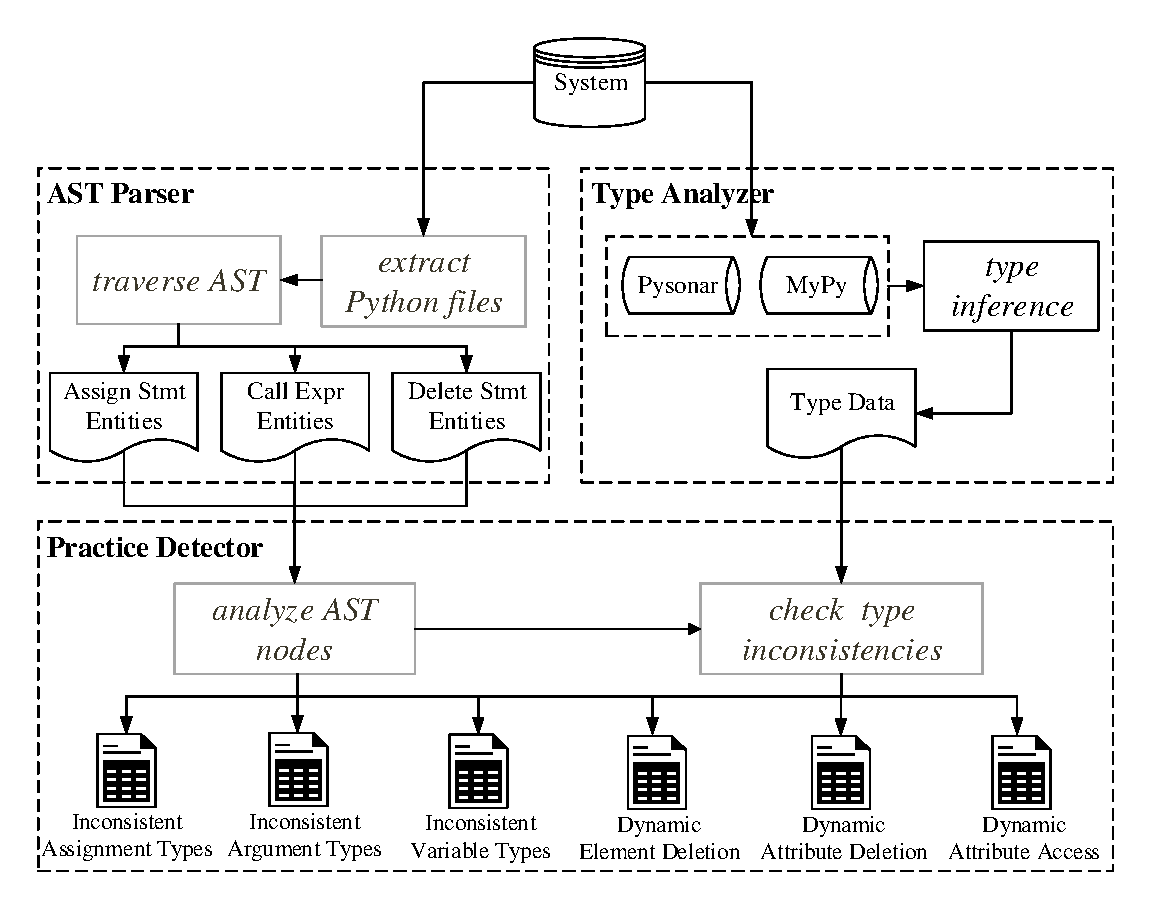
\includegraphics[width=1.0\linewidth]{figures/components.pdf}\vspace{-10pt}
	\caption{Identification of Dynamic Type-Aware Practices}\label{fig:components}
\end{figure}
% !TeX root = ../main.tex

\section{Study Design}\label{sec:setup}

\subsection{Research Questions}

Given that developers perform dynamic type-aware practices in Python programs but some of them are not the best solutions, it is unclear why developers use the risky type-aware practices and whether their usage correlates with increased likelihood of bug occurring.
With the goal of understanding the risky dynamic type-aware practices in Python systems, this study investigates how many dynamic type-aware practices exist in Python systems, how they are introduced into Python systems by developers, and whether they are related to software bugs. More specifically, this study aims at addressing the following research questions:

\textbf{RQ1 (Presence of Dynamic Type-Aware Practices):} \emph{How many dynamic type-aware practices exist in Python systems?} First of all, this research question aims at investigating whether the studied practices are widespread in Python systems. 

\textbf{RQ2 (Intents of Dynamic Type-Aware Practices):} \emph{How are dynamic type-aware practices introduced into Python systems?} The second research question addresses whether the studied practices are introduced as soon as the code entity is created, or whether, instead, they are introduced in the context of specific maintenance activities during software evolution.

\textbf{RQ3 (Relationship with Bugs):} \emph{What is the relationship between dynamic type-aware practices and bugs?} Python does not have compile-time type checking, thus various problems would appear at runtime, especially type errors and attribute errors. The answer to this question will discover whether the methods affected by the studied practices are more prone to bug occurring.

Three research questions in this study are investigated in two perspectives: \emph{Quantitative Research} observes and summarizes real-world facts by mining concrete datasets in publicly available Python systems, and \emph{Qualitative Research} conducts a survey by inviting Python developers to fill out a questionnaire about their experiences and points of the studied practices.

\subsection{Quantitative Research}

\textbf{Subject Systems.} The subject systems of this research consist of 9 open-source Python systems. We selected these systems because they are well-known systems (with from 820 to 31.3K stars on GitHub) in different domains (e.g., library, application, framework) and are nontrivial projects (from 12.7KLOC to 180.0KLOC). All the systems are hosted in Git repositories and record associated issue trackers.

TABLE \ref{tab:subjects} reports for each of them the description of the system (column 2), the overall number of Python files (column 3), methods (column 4) and lines of code (column 5) in the version on January 1 2016, the number of commits (column 6) and issues (column 7) during the 2016-17 year. 
In this research, we analyze the characteristics of dynamic type-aware practices in the first version in 2016 and explore their effects on bug issues during the following two years, given that two years are sufficient for developers to discover most of the bugs. 

\begin{table*}
	\setlength{\tabcolsep}{3.6pt}
	\caption{Subject Systems Under Quantitative Research}
	\centering
	\vspace{-10pt}
	\label{tab:subjects}
	\begin{tabular}{llrrrrr}
		\hline
		\textbf{System}	& \textbf{Description}	& \textbf{\#Files} &\textbf{\#Methods} & \textbf{LOC} &\textbf{\tabincell{l}{\#Commits\\\emph{(2016-17)}}}	&\textbf{\tabincell{l}{\#Issues\\\emph{(2016-17)}}}\\
		\hline
		{\tt borg} & Deduplicating archiver with compression and authenticated encryption & 37& 879&12.7K&3,170 &2,985\\
		{\tt ralph} & Asset management system for data center and back office &302& 1,066& 23.1K&858 &1,065\\
		{\tt fabric} &Simple, Pythonic remote execution and deployment  &79& 826&13.6K &244&288 \\
		{\tt requests} & Python HTTP requests for humans & 84&775&19.5K& 1,126&1,257\\
		{\tt tornado} & Python web framework and asynchronous networking library &112 &3,080& 40.2K&520&615 \\
		{\tt ansible} & Radically simple IT automation platform & 372&2,772& 61.9K&14,085& 20,614\\
		{\tt ipython} & Official repository for IPython itself & 334& 3,012&65.6K&1,911&1,860 \\
		{\tt beets} & Music library manager and MusicBrainz tagger &145 &3,451& 48.1K&2,166& 991\\
		{\tt scikit-learn} & Machine learning in Python & 644&5,465&180.0K &2,082& 4,279\\
		\hline
	\end{tabular}
\end{table*}

\textbf{Detection of Dynamic Type-Aware Practices.} 
Based on the detection strategy of dynamic type-aware practices described in Section \ref{sec:detection}, the detection result of risky type-aware practices is reported for each system. 

In order to evaluate the detection accuracy, we manually inspected a part of detected examples to check whether they are real dynamic type-aware practices. The manual inspection was performed together when investigating how dynamic type-aware practices are introduced into systems for RQ2 (detailed in the following paragraphs). The result comes out that there are three examples (two from \emph{Inconsistent Variable Types} and one from \emph{Inconsistent Argument Types}) which are false positives in 356 reported examples. Three false positives come from the incorrect results of the type inference tools.

In addition, false negatives generated from the detection can hardly be evaluated, because the accurate types are not available unless achieving full test coverage. But this study aims at understanding the characteristics of the detected practices and is complemented by the result of qualitative research, thus the occurrence of false negatives would not produce big biases.


\textbf{Mining of Practice Introducing Commits.}
In order to investigate how and when dynamic type-aware practices are introduced into Python systems, we randomly selected a part of detected practice examples, mined the commits which introduced the examples into systems, and then analyzed the developers' intents of the commits. Finally, we successfully mined 353 examples of dynamic type-aware practices.

We assume that the first commit in which the studied example is present is its introducing commit. The introducing commit was identified as follows. First, we mined the evolution history of the analyzed system and identified the methods $M_{c}$ that were changed in each commit $c$. Second, we extracted all candidate commits $CC$, where each commit $c$ in $CC$ satisfies that $M_{c}$ contains the method $m$ where the studied example is located. Third, for each candidate commit $c$ in $CC$, we automatically detected the type-aware practices in the version of $c$. If the detection result showed that the method $m$ did not contain the example in $c$, $c$ was filtered out from $CC$. Fourth, as each commit in the remaining $CC$ may be the introducing commit of the example, we manually checked them in reverse order by evolution history and stopped until we found the commit that introduced the studied example. 

After having identified the introducing commit of a type-aware practice example, we then analyzed the developer's intent of this commit to explore why the example was introduced into the system. As a starting point, we consider the set of tags with different intents proposed by Paixao et al. \cite{b29} and Tufano et al. \cite{b30}. The final set of tags used in this study is presented in TABLE \ref{tab:tags}. ``Development'' was used when the example was inserted along with the whole method that contains it in early development stages. The other tags were used when the introducing commits were used for regular maintenance tasks.
The manual inspection of dynamic type-aware practice examples was completed by three Ph.D students and each example was traced and tagged by at least two students. After the individual manual inspection, the students' decisions differed in 9 out of 353 examples. For these examples, the tags were finally determined after three students had a discussion and decided by consensus.

\begin{table}
	\caption{Tags Assigned to the Introducing Commits of Dynamic Type-aware Practices}
	\centering
	\vspace{-10pt}
	\label{tab:tags}
	\begin{tabular}{ll}
		\hline
		\textbf{Tag} & \textbf{Intent of Commit}\\
		\hline
		Development & The commit occurs in the unstable development phase\\
		New Feature &The commit aims at implementing a new feature\\
		Enhancement &The commit aims at enhancing an existing feature\\
		Platform Update &The commit aims at updating for a new platform/API\\
		Refactoring &The commit aims at refactoring the system\\
		Bug Fixing &The commit aims at fixing a bug\\
		\hline
	\end{tabular}
\end{table}

When mining the introducing commits of detected examples, an example would be filtered out if it is recognized as not belonging to real dynamic type-aware practices (i.e., a false positive) or the students can not have an agreed conclusion about the intent after discussion.
This mining process was finished until we had successfully mined the introducing commits of 60 randomly selected examples for each type of dynamic type-aware practices (all examples would be covered if the total number of the detected examples is less than 60).


\textbf{Extraction of Bug Affected Methods.}
%In order to explore the relationship between type-aware bad practices and bugs, 
The investigation of RQ3 explores how many methods that are affected by dynamic type-aware practices are also affected by bugs. Therefore, for each subject system, we identified all bug-fixing commits during the 2016-2017 year and extracted the methods that were changed in these bug-fixing commits. The extracted methods are considered as the methods that are affected by bugs.

We used the approach proposed by \'{S}liwerski et al.\cite{b31} to identify bug affected methods. For a subject system, we extracted all bug reports from the issue tracker system and all commit messages from the commit log. A common practice among developers is describing bug ID and bug summary in commit message whenever they fix a bug, thus we extracted bug-fixing commits by linking commit messages with bug reports, which is finished by matching bug ID or bug summary. Finally, the changed methods in bug-fixing commits were identified as the methods affected by bugs. In this experiment, we considered all tracked issues with different labels instead of only the issues labeled with ``Bug'', because all labels of issues may be resulted from dynamic type-aware practices and we are uncertain what bias this labeling could introduce.

\begin{table*}[ht]
	\caption{Survey Results in Qualitative Research}
	\setlength{\tabcolsep}{1.5 pt}
	\centering
	\vspace{-10pt}
	\label{tab:surveyresults}
	\begin{tabular}{l|l|cccccc}
		\hline
		\textbf{Survey Questions}    & \textbf{Options} &\textbf{\tabincell{c}{Inconsistent \\Assignment Types}}  &  \textbf{\tabincell{c}{Inconsistent \\Argument Types}} &\textbf{ \tabincell{c}{Inconsistent \\Variable Types}} & \textbf{\tabincell{c}{Dynamic \\ Element Deletion}}& \textbf{\tabincell{c}{Dynamic \\Attribute Deletion}} & \textbf{\tabincell{c}{Dynamic\\Attribute Access}}\\
		\hline
		SQ2: Widely Performed& &30\%  & 24\%   &54\%& 7\% & 3\%  &  11\%\\
		\hline
		\multirow{6}{*}{SQ3: Introducing Intents}  & a. development & 78\%&61\%&61\%&67\%&60\%&72\%           \\
		& b. new feature&27\%&41\%&31\%&22\%&18\%&25\%   \\
		& c. enhancement &27\%&28\%&34\%&22\%&27\%&24\% \\
		& d. refactoring &21\%&20\%&21\%&21\%&15\%&20\%	\\
		& e. bug fixing &11\%&20\%&20\%&22\%&20\%&12\%	 \\
		\hline
		SQ4: Leading to Bugs&  & 67\% & 52\%   &65\%& 64\% &  65\% &55\% \\            
		\hline	
	\end{tabular}
\end{table*}

\subsection{Qualitative Research}
We collected a list of Python developers actively contributing to popular systems from GitHub. Initially, we contacted some professional developers and inquired about their points of dynamic type-aware practices. Most developers pointed out that they were very interested in our study, and sent us their suggestions and experiences about dynamic type-aware practices. Generally, they believed that the studied practices are bad practices in complex scenarios.

After summarizing the initial feedback from developers,  we designed a questionnaire to developers and asked the following questions about six types of dynamic type-aware practices:
\begin{itemize}
	\item 
SQ1. How many years of experience do you have in programming with Python?
	\item 
SQ2. Which types of practices do you widely perform in Python code?
	\item 
SQ3. When do you often introduce them into Python code?
	\item 
SQ4. Which types of practices have ever led to bug issues in your experience?
\end{itemize}

The goal of this survey is getting individual answers to our research questions from developers (SQ2 for investigating RQ1, SQ3 for investigating RQ2, and SQ4 for investigating RQ3).
We invited 367 developers to complete this questionnaire and 70 developers fully completed it in two weeks. 

From the answers to SQ1, the Python programming experience of the survey participants is distributed over: less than 3 years (23\%), 4-6 years (27\%), 7-10 years (30\%), and more than 10 years (20\%). The answers to SQ2-SQ4 are summarized in TABLE \ref{tab:surveyresults}. This result will be explained and discussed in the following section.







% !TeX root = ../main.tex

\section{Study Results}

\subsection{(RQ1) Presence of Dynamic Type-Aware Practices}

\begin{table*}[ht]
	\caption{Number of Dynamic Type-aware Practices in Subject Systems}
	\centering
	\vspace{-10pt}
	\label{tab:instances}
	\begin{tabular}{lcccccc}
		\hline
		\textbf{System} & \textbf{\tabincell{c}{Inconsistent\\Assignment Types}}&	\textbf{\tabincell{c}{Inconsistent\\Argument Types}}& \textbf{\tabincell{c}{Inconsistent\\Variable Types}} & \textbf{\tabincell{c}{Dynamic\\Element Deletion}} & \textbf{\tabincell{c}{Dynamic\\Attribute Deletion}}&\textbf{\tabincell{c}{Dynamic\\Attribute Access }}\\
		\hline
		{\tt borg} & 8 & 3 & 98 & 17 & 0 & 21\\
		{\tt ralph} & 71 & 0 & 13 & 3 & 0 & 88\\
		{\tt fabric} & 6 & 0 & 264 & 15 & 15 & 19\\
		{\tt requests} & 15 & 	0 & 129 & 17 & 0 & 34\\
		{\tt tornado} & 28 & 	7 & 52 & 26 & 5 & 42\\
		{\tt ansible} & 49 & 	6 & 338 & 71 & 1 & 126\\
		{\tt ipython} & 49 & 	9 & 379 & 49 & 6 & 96\\
		{\tt beets} & 45 & 	63 & 201 & 43 & 7 & 32\\
		{\tt scikit-learn} & 75 & 	11 & 983 & 21 & 19 & 101\\
		\hline
		Average & 38 & 11	 & 273	& 29&6 &62\\			
		\hline
	\end{tabular}
\end{table*}

\textbf{Quantitative Research Result.} 
TABLE \ref{tab:instances} presents the number of dynamic type-aware practices detected in the analyzed version of each subject system. Dynamic type-aware practices exist inconsistently in different systems. For example, the most common type of type-aware practices in {\tt ralph} is \emph{Dynamic Attribute Access}, while the most common type in other systems is \emph{Inconsistent Variable Types}. The fact is that one type of dynamic type-aware practices usually gathers together in a system, which is caused by developers' individual coding habits.

Generally, \emph{Inconsistent Variable Types} is the most common type of dynamic type-aware practices, where there are as high as 273 examples in a Python system on average. The fact is that \emph{Inconsistent Variable Types} examples are usually closely linked, because a variable with inconsistent types would propagate to many other variables (e.g., the variables whose values are dependent on it). Therefore, the key of the refactoring of \emph{Inconsistent Variable Types} examples is identifying the root one which propagates the inconsistent types to other variables. Furthermore, we also inspected the inconsistent type sets in detected examples. We discovered that most examples are generated by the combination of \textit{string} with other inconsistent types. It is often the case that the value of a variable is parsed from the user inputs and its type is determined by the sources of the inputs (e.g., XML files, database, command line).

On the contrary, \emph{Inconsistent Argument Types} and \emph{Dynamic Attribute Deletion} rarely occur in Python systems, with only 11 and 6 examples on average. Type annotation is added in Python after the introduction of Python3, which supports annotating the desired types of function arguments. The new feature reduces the misuse of function arguments thus reduces \emph{Inconsistent Argument Types} practices. \emph{Dynamic Attribute Deletion} is seldom performed by developers because they prefer to reserve no longer used attributes according to our observation.


\textbf{Qualitative Research Result.} 
The result of SQ2 in TABLE \ref{tab:surveyresults} shows which types of dynamic type-aware practices are widely used by developers in Python systems. 54\% of Python developers widely perform \emph{Inconsistent Variable Types} practices, because ``duck typing is a widely-used Python idiom'' as they claimed. This finding is consistent with the result of quantitative research. 
Many developers do not perform \emph{Dynamic Attribute Access} widely and they explained that: ``a valid reason of visiting an attribute via reflection is when they write meta code''.
In addition, only 7\% and 3\% of Python developers often use \emph{Dynamic Element Deletion} and \emph{Dynamic Attribute Deletion}, respectively.   


\textbf{Summary.} Generally, \emph{Inconsistent Variable Types} is the most common type of dynamic type-aware practices, while \emph{Dynamic Attribute Deletion} rarely occurs in Python systems.

\subsection{(RQ2) Intents of Dynamic Type-Aware Practices}

\textbf{Quantitative Research Result.}
Grouped by the intents behind the introduction of dynamic type-aware practices, TABLE \ref{tab:introduction} reports the number of commits which introduced dynamic type-aware practice examples into each system according to our mining, inspection, and classification. 
In the table, 60 randomly selected examples were analyzed for each type of dynamic type-aware practices, while only 53 examples of \emph{Dynamic Attribute Deletion} in total were detected in subject systems thus we analyzed all of them. The examples for which the intents are not clear were left out of the analysis.

In total, most of the dynamic type-aware practices were introduced into systems during development phase (accounting for above half of the cases), followed by enhancing an existing feature, introducing a new feature to the system, fixing bugs, performing refactoring and platform update, respectively. Furthermore, we noticed that a commit would introduce multiple examples of dynamic type-aware practices in some cases. For example, a commit that introduced an \emph{Inconsistent Argument Types} example by adding a function call with an inconsistent argument type also introduced \emph{Inconsistent Variable Types} examples due to inconsistent types used in the called function.


When considering the most common intents behind dynamic type-aware practices, i.e., development, enhancement and new feature, this is expected because dynamic type-aware practices are highly useful for rapid development and are also generated for adding complexity followed by feature upgrade. On the contrary, dynamic type-aware practices are seldom used for bug fixing or refactoring. It implies that the studied practices are easy to perform but are not easy to maintain the system. 



\begin{table*}[ht]
	\caption{Number of commits that introduced dynamic type-aware practices into subject systems grouped by different intents}
	\centering
	\vspace{-10pt}
	\label{tab:introduction}
	\begin{tabular}{lcccccccc}
		\hline
		\textbf{Practice} &\textbf{Development} & \textbf{New Feature}&\textbf{Enhancement}&\textbf{Platform Update}&\textbf{Refactoring}&\textbf{Bug Fixing} & \textbf{Total}\\
		\hline
		Inconsistent Assignment Types&47& 4 &4 &0& 2&3&60\\
		Inconsistent Argument Types&44 &3& 9 &1 &1 &2&60\\
		Inconsistent Variable Types&21 &4 &17 &0& 3& 5&60\\
		Dynamic Element Deletion&35& 6 &15 &0 &2& 2&60\\
		Dynamic Attribute Deletion&47& 3 &0 &0& 2 &1 &53\\
		Dynamic Attribute Access&41&10&6 &0& 2 &1&60\\		
		\hline
	\end{tabular}
\end{table*}

\begin{table}[htbp]
	\centering
	\setlength{\tabcolsep}{3.6pt}
	\caption{Ratios of methods which contain dynamic type-aware practices in all system methods and in bug affected methods}
	\vspace{-10pt}
	\label{tab:bug}
	\begin{tabular}{lcccccc}
		\hline
		\multirow{2}{*}{\textbf{System}}&\multicolumn{3}{c}{\textbf{All System Methods}} &\multicolumn{3}{c}{\textbf{Bug Affected Methods}}\\
		\cmidrule(lr){2-4}  \cmidrule(lr){5-7} 
		& \textbf{\textit{\#Total}}& \textbf{\textit{\#Practice}}& \textbf{\textit{Ratio}} & \textbf{\textit{\#Total}}& \textbf{\textit{\#Practice}}& \textbf{\textit{Ratio}} \\
		\hline
		{\tt borg} &879&64	&7.3\%&42&7	&16.7\%\\
		{\tt ralph} &1,066&86&8.1\%&154&31	& 20.1\%\\
		{\tt fabric} &826&121&14.6\%&17&10	&58.9\%	\\
		{\tt requests} &775&87&11.2\%&49&11&22.4\%	\\	
		{\tt  tornado} &3,080&97 &3.1\%&84&6	&7.1\%\\
		{\tt ansible} &2,772&269&9.7\%&1,079&184	&17.1\%\\
		{\tt ipython}&3,012&258&8.6\%&129&17&	13.2\%\\	
		{\tt beets} &3,451&200&5.8\%&358&43 & 12.0\%\\
		{\tt scikit-learn} &5,465&406&7.4\%&1,500&165&	11.0\%\\
		\hline
	\end{tabular}
\end{table}

\textbf{Qualitative Research Result.}
The survey result of SQ3 in TABLE \ref{tab:surveyresults} presents when developers introduce dynamic type-aware practices into Python systems. Generally, Python developers introduce dynamic type-aware practices mainly during development phase (accounting for from 60\% to 78\% of developers), which agrees with the finding from our quantitative research. Developers explained that they ``would like to ensure loose typing and dynamic behaviors'' for rapid development. They admitted that ``some of the ways are not pythonic at all, but reduce many of the downsides of Python compared with static typing''. Developers also would like to perform these practices during software maintenance including adding new feature, feature enhancement, and refactoring. It is slightly different with the quantitative research findings. Developers explained that it often happens when they implement complex functions. The other intents are seldom mentioned by developers, thus are not presented in the table.


\textbf{Summary.} 
Dynamic type-aware practices are introduced by developers into Python systems mainly during early development phase, followed by during software maintenance phase including adding new feature and feature enhancement.




\begin{table*}[ht]
	\centering
	\setlength{\tabcolsep}{3.6pt}
	\caption{Result of Fisher's exact test (\textit{p}-value) and the odds ratio ($OR$)}
	\vspace{-10pt}
	\label{tab:fishertest}
	\begin{tabularwithnotes}{lcccccccccccccc}
		{
			\tnote[]{The number in bold indicates that there is a significant positive relationship between dynamic type-aware practices and bugs ($p$-value$<$0.05 and $OR$$>$1)}
		}
		\hline
		\textbf{System}& \multicolumn{2}{c}{\textbf{\tabincell{c}{Inconsistent\\Assignment Types}}}&	\multicolumn{2}{c}{\textbf{\tabincell{c}{Inconsistent\\Argument Types}}}& \multicolumn{2}{c}{\textbf{\tabincell{c}{Inconsistent\\Variable Types}}} & \multicolumn{2}{c}{\textbf{\tabincell{c}{Dynamic\\Element Deletion}}} & \multicolumn{2}{c}{\textbf{\tabincell{c}{Dynamic\\Attribute Deletion}}}&
		\multicolumn{2}{c}{\textbf{\tabincell{c}{Dynamic\\Attribute Access }}} &\multicolumn{2}{c}{\textbf{Total}} \\
		\cmidrule(lr){2-3}\cmidrule(lr){4-5}\cmidrule(lr){6-7}\cmidrule(lr){8-9}\cmidrule(lr){10-11}\cmidrule(lr){12-13}\cmidrule(lr){14-15}
		&\textbf{\textit{p}-value} & \textbf{\textit{OR}} &\textbf{\textit{p}-value} & \textbf{\textit{OR}}&\textbf{\textit{p}-value} & \textbf{\textit{OR}}&\textbf{\textit{p}-value} & \textbf{\textit{OR}}&\textbf{\textit{p}-value} & \textbf{\textit{OR}}&\textbf{\textit{p}-value} & \textbf{\textit{OR}}&\textbf{\textit{p}-value} & \textbf{\textit{OR}}\\
		\hline
		{\tt borg} &-&-&-&-&-&-&-&-&-&-&-&-&9.81E-02& 2.05	\\
		{\tt ralph} &-&-&-&-&-&-&-&-&-&-&\textbf{8.42E-05}&\textbf{2.95}&\textbf{9.07E-05}&\textbf{2.65}	\\
		{\tt fabric} &-&-&-&-&\textbf{1.98E-06}&\textbf{12.03}&-&-&-&-&-&-&\textbf{5.63E-06}&\textbf{9.97}\\
		{\tt requests} &-&-&-&-&\textbf{1.46E-03}&\textbf{4.17}&-&-&-&-&-&-&\textbf{4.08E-02}&\textbf{2.17}	\\	
		{\tt  tornado} &-&-&-&-&3.82E-01&1.57&3.07E-01&1.88&-&-&6.89E-01&1.17&6.34E-01&1.24\\
		{\tt ansible} &\textbf{2.66E-03}&\textbf{5.06}&-&-&\textbf{3.73E-14}&\textbf{4.39}&\textbf{2.77E-05}&\textbf{3.39}&-&-&\textbf{1.15E-05}&\textbf{2.67}&\textbf{2.50E-21}&\textbf{3.50}\\
		{\tt ipython}&\textbf{3.33E-02}&\textbf{3.71}&-&-&1.76E-01&2.10&1.68E-01&0&-&-&5.80E-01&1.19&1.07E-01&1.50\\	
		{\tt beets} &\textbf{3.79E-03}&\textbf{3.41}&-&-&\textbf{1.67E-04}&\textbf{2.60}&\textbf{3.06E-02}&\textbf{2.31}&-&-&4.14E-01&0.46&\textbf{1.29E-04}&\textbf{2.00}\\
		{\tt scikit-learn} &6.44E-01&1.18&-&-&\textbf{7.48E-03}&\textbf{1.40}&1.61E-02&0.12&-&-&\textbf{2.16E-02}&\textbf{1.76}&\textbf{2.79E-03}&\textbf{1.37}\\
		\hline
		Total & \textbf{7.82E-05}&\textbf{2.04}&5.30E-01& 0.74&\textbf{3.09E-22}& \textbf{2.15}&\textbf{1.18E-02} &\textbf{1.49}&1.65E-01& 0.44&\textbf{4.92E-08}& \textbf{1.87}&\textbf{1.98E-28}&\textbf{1.84}\\
		\hline
	\end{tabularwithnotes}
\end{table*}

\subsection{(RQ3) Relationship with Bugs}

\textbf{Quantitative Research Result.}
From the bug reports of subject systems, we mined the types of exceptions which were reported by users and developers. We found that the most common exceptions resulted from the bugs are \textit{TypeError} and \textit{AttributeError}. They account for 16.4\% and 14.2\% of the bug reports which record the occurred exceptions, respectively. This finding inspires our study of dynamic type-aware practices which may produce \textit{TypeError} and \textit{AttributeError}.

For each subject system, TABLE \ref{tab:bug} reports the ratios of the methods which contain dynamic type-aware practices in all methods and in bug affected methods. For each group of the methods, the table gives the total number of the methods (\emph{\#Total} columns), the number of the methods affected by dynamic type-aware practices (\emph{\#Practice} columns), the ratio of the affected methods (\emph{Ratio} columns, i.e., \emph{\#Practice}/\emph{\#Total}). The result reveals that in the methods which are affected by bugs, the ratios of dynamic type-aware practices are approximately 2 or 3 times higher than the ratios in all methods. We then hypothesize that certain types of dynamic type-aware practices are highly related with bugs in Python systems.

We then examined the hypothesis by applying Fisher's exact test and the odds ratio ($OR$)\cite{b32} to examine the association between dynamic type-aware practices and bugs. The test classifies all methods into four groups: (1) the methods not affected by dynamic type-aware practices or bugs;  (2) the methods only affected by dynamic type-aware practices; (3) the methods only affected by bugs; (4) the methods affected by both dynamic type-aware practices and bugs. Based on the four groups of the methods, Fisher's exact test calculates the $p$-value for evaluating the correlation between the two ways of classification, i.e., dynamic type-aware practices and bugs. The $OR$ indicates the likelihood that an event (e.g., that a method is affected by bugs) occurs, where $OR$$>$1 indicates that bugs are more likely to occur inside the methods affected by dynamic type-aware practices and $OR$=1 indicates an equal probability. In this study, if Fisher's exact test result shows that the bugs occurred in the methods affected by dynamic type-aware practices significantly differ from those in the methods not affected by dynamic type-aware practices ($p$-value$<$0.05), we referred to the $OR$ value to examine whether the presence of dynamic type-aware practices is related with the presence of bugs ($OR$$>$1) or the absence of bugs ($OR$$<$1). 

TABLE \ref{tab:fishertest} reports the result of Fisher's exact test and the odds ratio towards each type of dynamic type-aware practices in each system. The cells of ``\_'' indicate that we think the datasets of dynamic type-aware practices are not sufficient enough to perform Fisher's exact test (i.e., the methods affected by dynamic type-aware practices are less than 20). The cells in bold indicate that there is a significant positive relationship between dynamic type-aware practices and bugs (i.e., $p$-value$<$0.05 and $OR$$>$1). We can see that the positive relationship is discovered in most of subject systems and most types of dynamic type-aware practices. This finding suggests that the methods affected by dynamic type-aware practices are more prone to bugs. The exceptions come from \emph{Inconsistent Argument Types} and \emph{Dynamic Attribute Deletion}, because these dynamic type-aware practices are seldom performed by developers in subject systems.

\textbf{Qualitative Research Result.} 
The last rows of TABLE \ref{tab:surveyresults} report the survey result of SQ4. The astonishing truth is that although dynamic type-aware practices are often introduced into Python systems for particular programming tasks, most of the developers (ranging from 52\% to 67\%) have ever encountered bug issues caused by them. Developers explained that these practices are ``safe in most cases, but may induce maintenance issues'' in complex scenarios during evolution. For example, the \emph{Inconsistent Assignment Types} example in Section \ref{sec:intro} was reported an issue in bug reports. For refactoring, \emph{module\_name} in the first statement was renamed to \emph{api\_to\_module} and the last statement was changed to ``\textit{module\_name=api\_to\_module[api]}'', which makes the code easier to understand. Developers suggested that ``never use the same variable name for two things, even if it's the same type''.

Among all types of dynamic type-aware practices, developers reflected that \emph{Dynamic Attribute Deletion} is more related to bug occurring than other types. This finding is expected because dynamically deleting an attribute affects the operations on all related instances around the whole system. In addition, for the practices of inconsistent types, they said ``it can be a bit error prone when handling different types in the variables'' and they suggested to ``have the type contract explicitly in the documentation''.


\textbf{Summary.}
Most types of dynamic type-aware practices have a significant positive correlation with bugs in Python systems. More than 52\% of developers have realized that dynamic type-aware practices are prone to bugs.
% !TeX root = ../main.tex

\section{Discussion}

\subsection{Threats to Validity}
\textbf{Accuracy of Type Inference Tools.}
Static type inference for Python is highly challenging, because Python systems heavily utilize external API functions and objects can be dynamically mutated in different execution paths. We combined the results of Pysonar2 and Mypy to detect dynamic type-aware practices. However, the tools still exhibit inherent limitations, because they infer data types statically and can not cover all possible dynamic behaviors, which reduces the detection accuracy of dynamic type-aware practices. In fact, this study aims at investigating the coding practices performed by developers, not the problematic usage performed by users. It means that we expect to detect the practices which behave risky statically, not dynamically.

\textbf{Identification of Instance Introducing Commits.} 
In order to identify the commit that introduced a practice example, we first extract all the candidate commits which change the method that contains the example, and then check the candidate commits one by one. However, an example may be introduced when the commit changes the code outside of the method that contains it. For example, in an assignment statement where the new value of the variable comes from the return value of a function, \emph{Inconsistent Assignment Types} occurs when  a commit changes the return value with an inconsistent type in the function. We assume that the occurrence of this case is limited. 


\textbf{Selection of Subjects.} 
9 Python systems and 70 Python developers are selected in this study. We are aware that the study results are biased by the selection of these subjects and we cannot generalize the results of this study to a wider range of subjects.
As a future work, the study would be repeated across different systems and different developers so that the understanding of dynamic type-aware practices can be calibrated. More importantly, we expect to discover and analyze more types of risky practices from the future study.


\subsection{Lessons From Our Study}

\textbf{Developers follow different type-aware coding conventions.} An interesting finding from the survey is that developers give inconsistent answers to the questions. For example, 11\% of developers answered that they commonly use \emph{Dynamic Attribute Access} in Python systems, while some developers said such practices are really error-prone and a class should never have to visit an attribute via reflection. This is caused from different coding conventions followed by these developers. As we can see from the result in TABLE \ref{tab:instances}, the occurrences of each type of dynamic type-aware practices are not consistent among different systems. We find that some developers prefer developing Python systems in the way of static typing through type annotation, as they think static typing benefits maintenance tasks. We can also find most developers prefer dynamic typing in many programming tasks, as they believe dynamic typing speeds up development. 


\textbf{Dynamic type-aware practices are useful but dangerous.} As mentioned above, developers have widespread debate over the choice between dynamic typing and static typing. The result of this study gives hints about this topic, which benefits language design.

The result of RQ3 in this paper suggests that the misuse of dynamic type-aware practices leads to maintenance issues. Particularly, TABLE \ref{tab:surveyresults} reveals that more than half of developers experienced bugs caused by the studied practices. According to the feedback from some developers, they are aware that many dynamic type-aware practices are not the best solutions, which reduces software quality. They also claimed that one of the things they are always thinking about when developing with Python is the type of a variable and conveying complex types in the documentation. However, developers admitted they still do this a lot. The results of RQ1 and RQ2 also reveal that the dynamic type-aware practices are widely adopted by developers in different programming tasks. Developers explained that dynamic typing is actually a benefit to software development; e.g., dynamic typing allows to use implicit interfaces rather than explicit ones. In summary, our study suggests that dynamic typing is vital but threatening.

\textbf{Dynamic type-aware practices can be improved.} Faced with the detected dynamic type-aware practices, it requires tools for improving these practices. In fact, most of dynamic type-aware practices can be justified depending on a specific context for code readability. For example, 
\emph{Inconsistent Assignment Types} can be improved by not multiplicating intermediate variables; 
\emph{Inconsistent Argument Types} can be improved by mimicking function overloading in a data-driven programming paradigm; 
\emph{Inconsistent Variable Types} can be improved by performing type checks (e.g., by calling \textit{type} or \textit{isinstance} function) before the operations;
\emph{Dynamic Element Deletion} and \emph{Dynamic Attribute Deletion} can be improved by checking the existence of the object before the deletion;
\emph{Dynamic Attribute Access} can also be improved by providing a default value for the case that the attribute is non-existant.

In addition, there are some common strategies of reducing bugs caused by dynamic type-aware practices. 
\begin{itemize}
\item 
\textbf{Test, Test, Test.} Given that dynamic type-aware practices mainly occur during development phase according to the result of RQ2, developers suggested that ``all downsides of dynamic typing languages prove that strong testing is required to validate the program''. The idea is making sufficient tests and keeping test coverage high.
\item 
\textbf{Using ``try...except...''.} Python developers tend to use ``try...except...'' operations to catch the exceptions, over writing code that seeks to avoid exceptions in the first place. Sometimes developers even deliberately do not handle the exceptions.  For example, \emph{Dynamic Attribute Access} practices are protected by ``try...except \textit{AttributeError}...'' rather than setting a default value of \textit{None}. The reason is that it is a way of signaling invalid input to the caller when it is not appropriate.
\item 
\textbf{Type Annotation.} When developing with Python, developers responded that they ``do not have a hard requirement on documentation but have a hard requirement on defining the types of arguments and return values of a function''. If the type contract is explicitly annotated in the documentation, it should be fairly straight forward to check that all cases are covered in code review.
\end{itemize}
% !TeX root = ../main.tex

\section{Related Work}

\noindent{\bf Empirical Studies of Dynamic Features.}
The study of dynamic feature usage has been addressed by researchers in many programming languages, including Smalltalk\cite{b6}, JavaScript\cite{b3}, AspectJ\cite{b7}, and Python\cite{b5,b8}. Holkner and Harland\cite{b5} carried out the first study on the usage of dynamic features in Python. They traced the occurrences of dynamic feature code and found the behaviors of dynamic features mainly occur during program startup. Later in 2014, {\AA}kerblom et al. \cite{b8} reported a similar study but demonstrated that dynamic activities neither prominently occur at startup phases nor are buried in the library. These studies suggest that dynamic features are an important part in programming tasks.

Negative aspects of dynamic features were also found during maintenance phase, especially in JavaScript\cite{b9} and Python\cite{b4,b19}. 
Park et al. \cite{b9} found that extremely dynamic features of JavaScript make it difficult to analyze Web applications statically, particularly resulting in too many false positives. 
Wang et al. \cite{b4} pointed out that dynamic feature code is generally error-prone and unpleasant to maintain in Python systems, which makes dynamic feature code changeable during evolution. 
Chen et al. \cite{b19} found that the misuse of dynamic features introduces bugs in Python systems and the bugs are often fixed by adding a check or adding an exception handling. 
The above studies of dynamic features demonstrate that the misuse of dynamic features poses threats to software maintenance. In this paper, the study addresses the misuse of Python dynamic features on its dynamic type system, including dynamic typing and dynamic object changes.


\noindent{\bf Evaluation of Dynamic Type Systems.}
The question of whether or not a kind of type system has any benefit is not indisputable. Multiple studies have performed the comparison between dynamic and static type systems along different dimensions, including development productivity \cite{b21,b25} , code usability\cite{b26}, and code quality \cite{b10,b28}.
Stuchlik and Hanenberg \cite{b21} compared statically and dynamically typed languages (i.e., Java and Groovy) in the relationship between type casts and development time. Their experiment was performed on 21 subjects who performed programming tasks using two programming languages, and discovered that the dynamically typed group solved the programming tasks significantly faster for most tasks.
Kleinschmager et al. \cite{b25} reported a similar experiment and showed rigorous evidence that static type systems are indeed beneficial to maintenance activities, except for fixing semantic errors.		
Mayer et al. \cite{b26} conducted a controlled experiment where 27 subjects performed programming tasks on an undocumented API with a static type system and a dynamic type system. Their results show that for three out of five tasks of using undocumented software, programmers had faster completion times using a static type system.
Gao et al. \cite{b10} evaluated the code quality benefits that static type systems provide to JavaScript codebases. The central finding is that using static type systems (i.e., Flow and TypeScript) could have prevented 15\% of the public bugs.
Ray et al. \cite{b28} gathered a very large dataset from GitHub to study the effects of language features on software quality. They reported that language design does have a significant, but modest effect on software quality. Especially, they concluded that static typing is somewhat better than dynamic typing.
		
Since researchers have valid arguments for a kind of type system, the conclusions about which kind of type system is better contradict each other. This study analyzes six types of dynamic type-aware practices in Python systems, which reveals the positive and negative roles of dynamic type system.
		
		
\noindent{\bf Detection of Type-Aware Bugs and Bad Practices.}	
Owing to the lack of type declarations in Python and other dynamically typed languages, it is common to appear type-aware issues (caused by bad practices or bugs) but is hard for developers to fix them. The key to detecting and fixing type-aware bad practices or bugs is type inference. Recent work on type inference to dynamically typed languages has adopted type hints to improve type inference. Xu et al. \cite{b14} extracted type hints from attribute accesses and variable names. They correlated these type hints through probabilistic inference, and eventually converged on probabilities of variable types in Python programs. Similarly, Milojkovi{\'c} et al. \cite{b20} exploited type hints in methods, including argument names and type annotations, to augment the performance of a static type inference algorithm.

Due to the lack of compile-time type checking, type errors in dynamic languages may remain unnoticed. Xu et al. \cite{b15} developed a predictive analysis engine for Python programs. It supports adding assertions for type bug detection, including subtype assertion and attribute assertion. Chen et al.\cite{b17} presented a constraint framework based on Python's structural equivalence type system, where constraints are extracted from source code via static analysis and are used to check bugs. Currently, the techniques of detecting type bugs in dynamic languages are still restricted to the size of analyzed systems.

Bad coding practices are widely analyzed to provide hints of refactoring tasks. Type-aware bad practices were also mentioned in other researches\cite{b11,b2,b1}. 
Gong et al.\cite{b11} mined and checked three type-related rules for occurrences of multi-event runtime patterns in JavaScript, including  ``too many arguments'', ``accessing the undefined property'' and ``concatenate undefined and a string''. 
Pradel et al. \cite{b2} classified all type coercions in JavaScript into likely harmless and potentially harmful coercions, and summarized the bad usage and the ugly usage of type coercions. 
Similar to our work, Pradel et al. \cite{b1} also presented a mostly dynamic analysis that warns developers about variables, properties, and functions that have inconsistent types in JavaScript. In this paper, we extend their work on dynamic type-aware practices. First, their work only focused on inconsistent types, while our study covers six types of type-aware practices based on dynamic typing features. Second, their work aimed at detecting inconsistent types in JavaScript programs without analyzing detailed effects of inconsistent types. This paper provides empirical evidence about how dynamic type-aware practices are introduced by developers into systems and how they benefit or reduce software development and maintenance.







	


% !TeX root = ../main.tex

\section{Conclusions}

Given that type errors commonly occur in dynamically typed languages such as Python, the misuse of the free typing discipline may produce hidden bugs and reduce software quality. In this paper, we studied six types of risky type-aware practices performed by developers in Python programs. We carried out a study, which consists of quantitative research and qualitative research, to investigate the characteristics and the effects of dynamic type-aware practices in Python systems. The results show that: (1) \emph{Inconsistent Variable Types} is the most common type of dynamic type-aware practices, while \emph{Dynamic Attribute Deletion} rarely occurs in Python systems; (2) dynamic type-aware practices are introduced by developers into Python systems mainly during early development phase; (3) most types of dynamic type-aware practices have a significant positive correlation with bug occurring in Python systems, and more than 52\% of developers have realized it. These findings also imply that: (1) developers follow different type-aware coding conventions; (2) dynamic type-aware practices are useful but dangerous; (3) dynamic type-aware practices can be improved.

Based on this study of dynamic type-aware practices, we suggest that developers should restrict their way of using dynamic typing discipline, and encourage researchers and practitioners to develop effective tools to improve dynamic type-aware practices.



\begin{thebibliography}{00}
\bibitem{b1} M. Pradel, P. Schuh, and K. Sen, ``TypeDevil: Dynamic type inconsistency analysis for JavaScript,'' Proceedings of the 37th International Conference on Software Engineering, vol. 1, pp. 314��C324, 2015.	
\bibitem{b2} S. Burckhardt, D. Leijen, and J. Protzenko, ``The good, the bad, and the ugly: An empirical study of implicit type conversions in JavaScript,'' LIPIcs-Leibniz International Proceedings in Informatics, vol. 37. Schloss Dagstuhl-Leibniz-Zentrum fuer Informatik, 2015.
\bibitem{b3} G. Richards, S. Lebresne, B. Burg, and J. Vitek, ``An analysis of the dynamic behavior of JavaScript programs,'' ACM SIGPLAN Notices, vol. 45, no. 6, pp. 1-12. ACM, 2010.
\bibitem{b4} B. Wang, L. Chen, W. Ma, Z. Chen, and B. Xu, ``An empirical study on the impact of Python dynamic features on change-proneness,'' Proceedings of the 27th International Conference on Software Engineering and Knowledge Engineering, pp. 134��C139, 2015.
\bibitem{b5} A. Holkner and J. Harland, ``Evaluating the dynamic behaviour of Python applications,'' Proceedings of the Thirty-Second Australasian Conference on Computer Science, vol. 91. Australian Computer Society, Inc., 2009.
\bibitem{b6} O. Calla\'{u}, R. Robbes, . Tanter, and D. Rthlisberger, ``How (and why) developers use the dynamic features of programming languages: the case of Smalltalk," Empirical Software Engineering, 18.6 (2013): 1156-1194.
\bibitem{b7} B. Dufour, C. Goard, L. Hendren, O. de Moor, G. Sittampalam, and C. Verbrugge, ``Measuring the dynamic behaviour of AspectJ programs,'' ACM SIGPLAN Notices, 39.10 (2004): 150-169.
\bibitem{b8} B. {\AA}kerblom, J. Stendahl, M. Tumlin, and T. Wrigstad, ``Tracing dynamic features in Python programs,'' Proceedings of the 11th Working Conference on Mining Software Repositories, pp. 292-295. ACM, 2014.
\bibitem{b9} J. Park, I. Lim, and S. Ryu, ``Battles with false positives in static analysis of JavaScript web applications in the wild,'' Proceedings of the IEEE/ACM International Conference on Software Engineering Companion, pp. 61-70. IEEE, 2016.
\bibitem{b10} Z. Gao, C. Bird, and E. T. Barr, ``To type or not to type: quantifying detectable bugs in JavaScript,'' Proceedings of the 39th International Conference on Software Engineering, pp. 758-769. IEEE, 2017.
\bibitem{b11} L. Gong, M. Pradel, M. Sridharan, and K. Sen, ``DLint: Dynamically checking bad coding practices in JavaScript,'' Proceedings of the 2015 International Symposium on Software Testing and Analysis, pp. 94-105. ACM, 2015.
%\bibitem{b12} Y. Liu, C. Xu, S.-C. Cheung, and V. Terragni, ``Understanding and detecting wake lock misuses for Android applications,'' Proc. 2016 24th ACM SIGSOFT Int. Symp. Found. Softw. Eng. - FSE 2016, pp. 396��C409, 2016.
%\bibitem{b13} G. Mezzetti, A. Mller, and F. Strocco, ``Type Unsoundness in Practice: An Empirical Study of Dart,'' Dsl16, pp. 13��C24, 2016.
\bibitem{b14} Z. Xu, X. Zhang, L. Chen, K. Pei, and B. Xu, ``Python probabilistic type inference with natural language support,'' Proceedings of the 2016 24th ACM SIGSOFT International Symposium on Foundations of Software Engineering, pp. 607-618. ACM, 2016.
\bibitem{b15} Z. Xu, P. Liu, X. Zhang, and B. Xu. ``Python predictive analysis for bug detection," Proceedings of the 2016 24th ACM SIGSOFT International Symposium on Foundations of Software Engineering, pp. 121-132. ACM, 2016.
%\bibitem{b16} Vitousek M M, Kent A M, Siek J G, et al. Design and evaluation of gradual typing for Python[C]//ACM SIGPLAN Notices. ACM, 2014, 50(2): 45-56.
\bibitem{b17} L. Chen, B. Xu, T. Zhou, and X. Zhou, ``A constraint based bug checking approach for python," Proceedings of the 33rd Annual IEEE International In Computer Software and Applications Conference, vol. 2, pp. 306-311. IEEE, 2009.
%\bibitem{b18} Chen Z, Chen L, Ma W, et al. Understanding metric-based detectable smells in Python software: A comparative study[J]. Information and Software Technology, 2018, 94: 14-29.
\bibitem{b19} Z. Chen, W. Ma, W. Lin, L. Chen, Y. Li, and B. Xu, ``A study on the changes of dynamic feature code when fixing bugs: towards the benefits and costs of Python dynamic features," Science China Information Sciences, 61, no. 1 (2018): 012107.
\bibitem{b20} N. Milojkovi{\'c}, M. Ghafari, and O. Nierstrasz, ``Exploiting type hints in method argument names to improve lightweight type inference," Proceedings of the 25th International Conference on Program Comprehension, pp. 77-87. IEEE, 2017.
\bibitem{b21} A. Stuchlik and S. Hanenberg, ``Static vs. dynamic type systems: an empirical study about the relationship between type casts and development time," ACM SIGPLAN Notices, vol. 47, no. 2, pp. 97-106. ACM, 2011.
%\bibitem{b22} Milojkovic N, Ghafari M, Nierstrasz O. It's duck (typing) season![C]//Program Comprehension (ICPC), 2017 IEEE/ACM 25th International Conference on. IEEE, 2017: 312-315.
%\bibitem{b23} Spasojevic B, Lungu M, Nierstrasz O. A case study on type hints in method argument names in Pharo Smalltalk projects[C]//Software Analysis, Evolution, and Reengineering (SANER), 2016 IEEE 23rd International Conference on. IEEE, 2016, 1: 283-292.
%\bibitem{b24} M. T. Daly, V. Sazawal, and J. S. Foster, ``Work in progress: an empirical study of static typing in ruby'', 2009.
\bibitem{b25} S. Kleinschmager, R. Robbes, A. Stefik, S. Hanenberg, and E. Tanter, ``Do static type systems improve the maintainability of software systems? An empirical study,'' Proceedings of the 20th International Conference on Program Comprehension, pp. 153-162. IEEE, 2012.
\bibitem{b26} C. Mayer, S. Hanenberg, R. Robbes, {\'E}. Tanter, and A. Stefik, ``An empirical study of the influence of static
type systems on the usability of undocumented software,'' ACM SIGPLAN Notices, vol. 47, no. 10, pp. 683-702. ACM, 2012.
\bibitem{b27} L. A. Meyerovich and A. Rabkin, ``Empirical analysis of programming language adoption,'' ACM SIGPLAN Notices, 2013, 48(10): 1-18.
\bibitem{b28} B. Ray, D. Posnett, V. Filkov, and P. Devanbu, ``A large scale study of programming languages and code quality in github,'' Proceedings of the 22nd ACM SIGSOFT International Symposium on Foundations of Software Engineering, ACM, 2014, pp. 155��C165.
\bibitem{b29} M. Paixao, J. Krinke, D. Han, C. Ragkhitwetsagul, and M. Harman, ``Are developers aware of the architectural impact of their changes?," Proceedings of the 32nd IEEE/ACM International Conference on Automated Software Engineering, pp. 95-105. IEEE, 2017.
\bibitem{b30} M. Tufano, F. Palomba, G. Bavota, R. Oliveto, M. Di Penta, A. De Lucia, and D. Poshyvanyk, ``When and why your code starts to smell bad,'' Proceedings of the 37th IEEE International Conference on Software Engineering, vol. 1, pp. 403-414. IEEE, 2015.
\bibitem{b31} J. \'{S}liwerski, T. Zimmermann, A. Zeller, ``When do changes induce fixes?,'' ACM SIGSOFT Software Engineering Notes, vol. 30, no. 4, pp. 1-5. ACM, 2005.
\bibitem{b32} R. A. Fisher,``Statistical methods for research workers," Breakthroughs in Statistics, pp. 66-70. Springer, New York, NY, 1992.
\bibitem{b33} L. Eder, ``The inconvenient truth about dynamic vs. static typing,'' http://blog.jooq.org/2014/12/11/the-inconvenient-truth-about-dynamic-vs-static-typing,
December 2014.
\bibitem{b34} A. Janmyr, ``Static typing is the root of all evil,'' http://www.jayway.com/2010/04/14/static-typing-is-the-root-of-all-evil/, April 2010.
\bibitem{b35} ``Python'', https://www.python.org/.

\bibitem{b36} ``ipython'', https://github.com/ipython/ipython.
\bibitem{b37} ``tornado'', https://github.com/tornadoweb/tornado.
\bibitem{b38} ``scikit-learn'', https://github.com/scikit-learn/scikit-learn.
\bibitem{b39} ``django'', https://github.com/django/django.
\bibitem{b40} ``ansible'', https://github.com/ansible/ansible.
\bibitem{b41} ``Pysonar2'', https://github.com/leafgray/pysonar2.
\bibitem{b42} ``Mypy'', http://mypy-lang.org/.

\end{thebibliography}

\end{document}
